\section{Results and Discussion}\label{Sec:Evaluation}

We evaluate the performance of our methods on the meshes of Fig.~\ref{fig:meshes}.
    
\begin{figure*}
    \centering%
    \def\svgwidth{\textwidth}%
    \fontsize{6pt}{5pt}\selectfont%
    \includesvg{figs/meshes}%
    \caption[Test Meshes]{
    $V$ denotes the number of vertices of the input mesh, $T$ the number of triangles and $M$ the number of meshlets coming from Meshoptimizer.
    Meshlets are visualized with randomized colors.
    }\label{fig:meshes}%
\end{figure*}%

\begin{table}
    \caption
    [Comparison for the \textit{Rock} mesh.]
    {    
    We compare the optimal Gurobi and SCIP solutions against the sub-optimal stuff.
    The CPU computation uses one thread per meshlet and was measured on an AMD Ryzen 9 7950X (16C/32T).    
    }\label{tab:StripifyTable}    
    {
    \centering    
    \footnotesize
\begin{tblr}[b]{lccc}
    \toprule                                        
                     & \textbf{Gurobi} & \textbf{SCIP}       & \textbf{ETA}\\
\midrule                                    
\textbf{computation time}     & 122.46\,s    & 8,122.56\,s & 10.52\,s   \\
\textbf{\acs{GTS} render time} & 1.58\,ms     & 1.58\,ms    & 0.59\,ms \\
\textbf{\acs{GTS} restarts}    & 123,784      & 123,784     & 185,480\\
\textbf{degenerate triangles} & 2,132      & 495,136     & 741,920\\
\textbf{additional meshlets}  & 1 / 12412   & 123  & 4 / 75,413\\
\bottomrule                                    
\end{tblr}


    }
\end{table}


\begin{figure}
    \includesvg[inkscapelatex=true]{figs/PDFTexFigure}
    \caption[Vector graphics with fonts rendered by latex]{You can use Latex to render the fonts.}\label{fig:latexfonts}
\end{figure}

\begin{figure}
    \includesvg[inkscapelatex=false]{figs/SVGFigure}
    \caption[Vector graphics with fonts directly taken from the file]{You can also use the fonts produced by the SVG file.}\label{fig:svgfonts}
\end{figure}

\begin{figure}
    \centering
    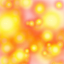
\includegraphics[width=\columnwidth]{imgs/img.png}
    \caption[Pixel graphics]{You can also directly include pixel graphics.}\label{fig:pixel}
\end{figure}

Tab.~\ref{tab:StripifyTable} and Tab.~\ref{tab:ListOfSymbols} compare our optimal 
method achieved with our other method
of Sec.~\ref{Sec:MainPart} with Gurobi and SCIP against the sub-optimal strip of our 
other implementation.
See Figs.~\ref{fig:latexfonts}, Figs.~\ref{fig:svgfonts}, and Figs.~\ref{fig:pixel} for different types of figures.
Here we test the acronyms.

% Test acronyms
First time we use a \ac{GPU}.
Next time, we use a \ac{GPU}.
Now, we even have multiple \acp{GPU}.
